% Компіляція: lualatex -shell-escape main.tex
\documentclass[12pt,a4paper]{article}

\usepackage{fontspec}
\usepackage{polyglossia}
\setdefaultlanguage{ukrainian}
\setmainfont{NewComputerModern10}
\setmonofont{Noto Sans Mono}[Scale=0.82]

\usepackage{amsmath,amssymb,booktabs,caption,enumitem,float,geometry,graphicx,hyperref,minted,microtype,tikz,xcolor,titlesec}
\usetikzlibrary{arrows.meta,positioning,shapes.geometric}
\geometry{left=2cm,right=2cm,top=2cm,bottom=2cm}
\setlength{\parindent}{1.25cm}
\setlength{\parskip}{0pt}
\setlength{\emergencystretch}{3em}
\linespread{1.0}
\usemintedstyle{vs}
\setminted{linenos,breaklines,frame=single,fontsize=\small,tabsize=4}
\captionsetup{font=small,labelfont=bf,labelsep=endash}
\titleformat{\section}{\normalfont\fontsize{14}{16}\selectfont\bfseries\centering}{\thesection.}{0.6em}{}
\titleformat{\subsection}{\normalfont\fontsize{12}{14}\selectfont\bfseries\centering}{\thesubsection.}{0.6em}{}
\titlespacing*{\section}{0pt}{1.4em}{0.65em}
\titlespacing*{\subsection}{0pt}{1.1em}{0.45em}

\newcommand{\studentName}{Давидчук А. М.}
\newcommand{\studentGroup}{ІО-41}
\newcommand{\recordBook}{4106}
\newcommand{\teacherName}{Баран Д. Р.}
\newcommand{\reportYear}{2026}

\newcommand{\imagepair}[3]{%
\begin{figure}[H]\centering
\begin{minipage}[t]{0.48\textwidth}\centering
\includegraphics[width=\linewidth]{#2}\\[-0.2em]
\small Landsat/ArcGIS
\end{minipage}\hfill
\begin{minipage}[t]{0.48\textwidth}\centering
\includegraphics[width=\linewidth]{#3}\\[-0.2em]
\small Bing Maps
\end{minipage}
\caption{#1}
\end{figure}}

\begin{document}
\pagenumbering{gobble}
\begin{titlepage}
  \begin{center}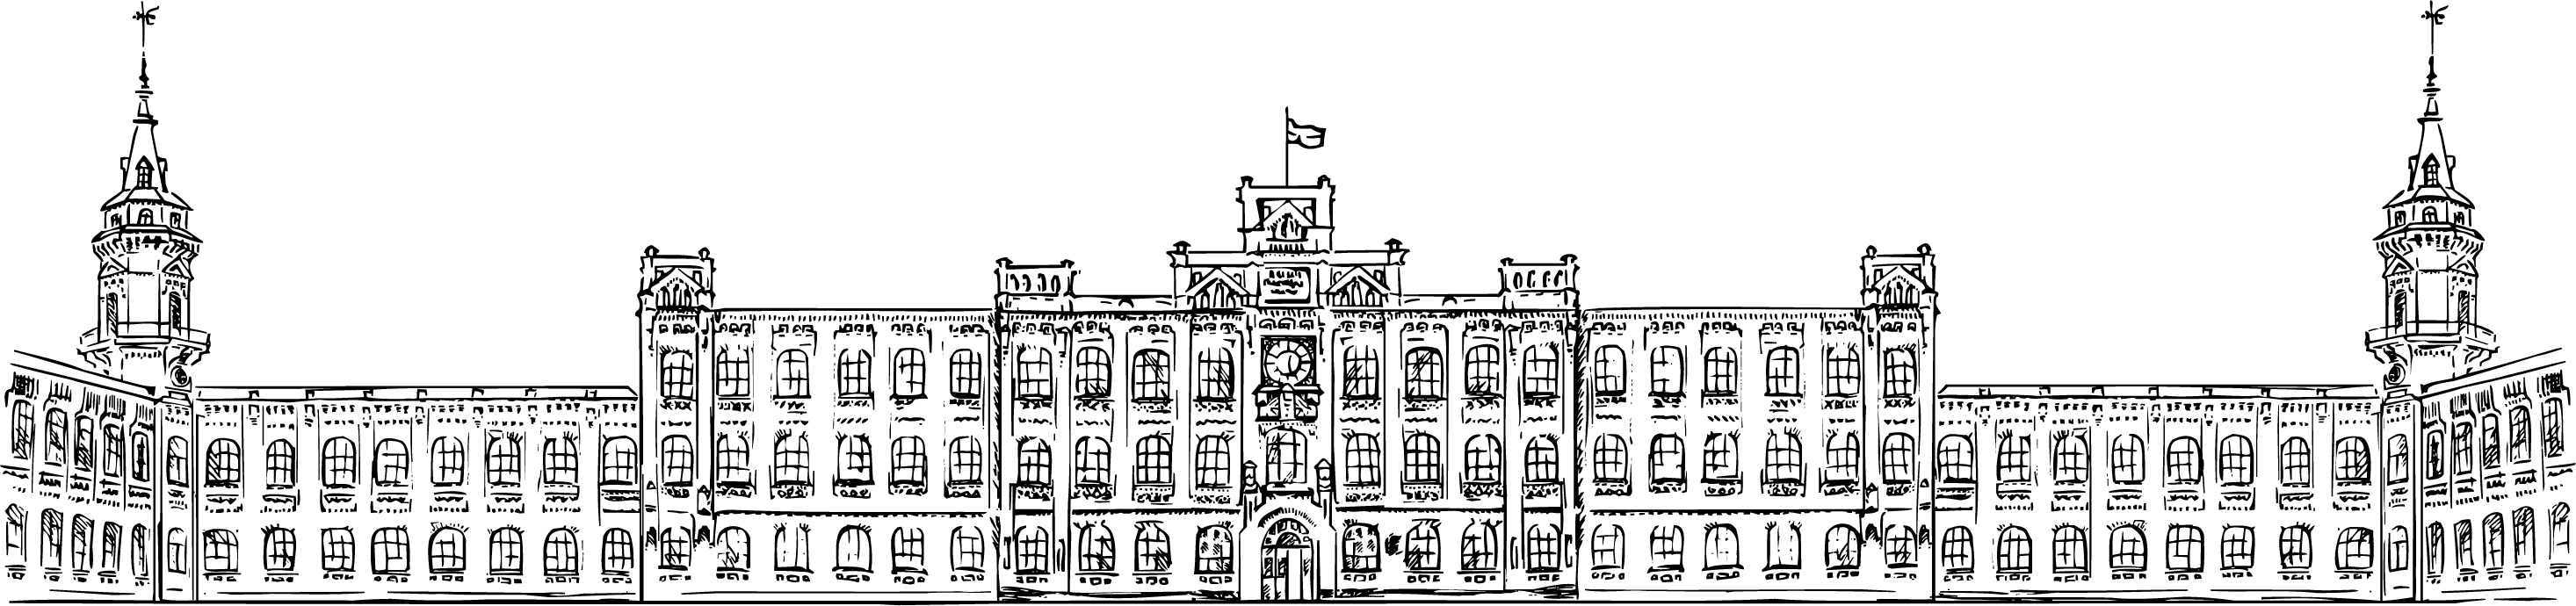
\includegraphics[width=0.7\textwidth]{../../../../../../templates/letterhead.png}\end{center}
  \begin{center}\large
    Національний технічний університет України\\
    «Київський політехнічний інститут імені Ігоря Сікорського»\\[1em]
    Факультет інформатики та обчислювальної техніки\\
    Кафедра обчислювальної техніки
  \end{center}
  \vfill
  \begin{center}
    \textbf{\LARGE Технології Computer Vision}\\[2em]
    \textbf{\Large Лабораторна робота №4}\\[0.7em]
    \parbox{0.9\textwidth}{\centering «Технології порівняння цифрових зображень»}
  \end{center}
  \vfill
  \begin{flushright}\begin{minipage}{0.48\textwidth}
    Виконав: студент 3 курсу ФІОТ,\\
    групи \studentGroup\\
    \textit{\studentName}\\
    Залікова книжка № \recordBook\\[1em]
    Перевірив: \textit{\teacherName}
  \end{minipage}\end{flushright}
  \vfill
  \begin{center}Київ --- \reportYear\end{center}
\end{titlepage}

\pagenumbering{arabic}
\section{Тема та мета роботи}
\noindent\textbf{Тема:} технології порівняння цифрових зображень.

\medskip
\noindent\textbf{Мета:} дослідити принципи та особливості практичного застосування технологій порівняння цифрових зображень для задач Computer Vision із використанням спеціалізованих програмних бібліотек.

\section{Завдання роботи}
Для виконання обрано \textbf{групу вимог 1} методичних рекомендацій. Необхідно:
\begin{enumerate}[leftmargin=*,itemsep=0.25em]
  \item використати два статичні знімки однієї ділянки земної поверхні, отримані з різних за якістю й оперативністю джерел;
  \item урахувати результати цифрової обробки зображень, отримані в ЛР2 та ЛР3, і підготувати зображення до порівняння;
  \item обрати метод виділення особливих точок і виконати порівняння однакових об'єктів на двох знімках;
  \item оцінити ймовірність ідентифікації як відношення кількості підтверджених особливих точок об'єкта до кількості придатних точок, що беруть участь у порівнянні;
  \item методами цифрової обробки зображень отримати ймовірність ідентифікації не гірше $0{,}9$.
\end{enumerate}

Об'єктом ідентифікації обрано територіальний об'єкт --- центральну частину головного кампусу КПІ. Порівнюються знімки Landsat/ArcGIS і Bing Maps. Методи глибинного навчання не використовуються.

\section{Математична модель}
Зображення переводяться у відтінки сірого, після чого локальний контраст вирівнюється методом CLAHE. На кожному зображенні детектор знаходить ключові точки
\begin{equation}
K=\{k_i=(x_i,y_i,s_i,\varphi_i)\},
\end{equation}
де $x_i,y_i$ --- координати, $s_i$ --- масштаб, $\varphi_i$ --- орієнтація точки. Для кожної точки обчислюється дескриптор $d_i$.

Пошук найближчих дескрипторів виконується алгоритмом $k$-NN для $k=2$. Відповідність приймається за ratio test, якщо
\begin{equation}
D(d_i,d_{j_1}) < \tau D(d_i,d_{j_2}),\qquad \tau=0{,}65,
\end{equation}
де $j_1,j_2$ --- перший і другий найближчі сусіди. Для ORB застосовується відстань Геммінга, для SIFT --- евклідова відстань.

Геометричний зв'язок між знімками задається гомографією
\begin{equation}
\lambda
\begin{bmatrix}x'\\y'\\1\end{bmatrix}
=H
\begin{bmatrix}x\\y\\1\end{bmatrix},
\qquad H\in\mathbb{R}^{3\times3}.
\end{equation}
Матриця $H$ оцінюється методом RANSAC. Відповідність вважається підтвердженою, якщо її похибка репроєкції не перевищує 4 пікселі.

Відповідно до ТЗ ймовірність ідентифікації визначено як
\begin{equation}
P_{id}=\frac{N_{inlier}}{N_{usable}},
\end{equation}
де $N_{usable}$ --- кількість відповідностей після ratio test, а $N_{inlier}$ --- кількість відповідностей, підтверджених RANSAC. Умова виконання завдання: $P_{id}\geq0{,}9$.

\section{Архітектура програмного рішення}
\begin{figure}[H]\centering
\begin{tikzpicture}[
  node distance=0.55cm and 0.6cm,
  block/.style={draw,rounded corners,align=center,minimum width=2.8cm,minimum height=0.8cm,fill=blue!7},
  arrow/.style={-{Latex[length=2mm]},thick}]
  \node[block] (input) {Landsat та Bing};
  \node[block,right=of input] (prep) {Grayscale\\та CLAHE};
  \node[block,right=of prep] (features) {ORB / SIFT\\точки й дескриптори};
  \node[block,below=of features] (match) {BFMatcher, $k=2$\\ratio test};
  \node[block,left=of match] (ransac) {RANSAC\\та гомографія};
  \node[block,left=of ransac] (out) {$P_{id}$, візуалізація\\і верифікація};
  \draw[arrow] (input)--(prep)--(features)--(match)--(ransac)--(out);
\end{tikzpicture}
\caption{Блок-схема алгоритму порівняння зображень}
\end{figure}

Після завантаження знімки незалежно проходять однакову попередню обробку. Для кожного досліджуваного методу будуються ключові точки та дескриптори. BFMatcher формує пари, ratio test видаляє неоднозначні відповідності, а RANSAC відкидає геометрично неузгоджені пари. За підтвердженими точками обчислюється гомографія, імовірність ідентифікації та візуалізація суміщення.

\section{Структура проєкту}
\begin{verbatim}
lab4/
|-- src/
|   |-- main.py
|   |-- landsat.png
|   `-- bing.png
|-- results/
|   |-- orb/
|   |-- sift/
|   `-- summary.csv
|-- requirements.txt
`-- docs/
    |-- main.tex
    `-- main.pdf
\end{verbatim}

\section{Результати виконання}
\subsection{Вхідні дані та підготовка}
\imagepair{Вхідні знімки центральної частини кампусу КПІ}{../src/landsat.png}{../src/bing.png}
\imagepair{Зображення після grayscale та CLAHE}{../results/orb/reference_preprocessed.png}{../results/orb/candidate_preprocessed.png}

Знімки мають різні розміри, деталізацію, колірний баланс і частково різне поле огляду. Тому порівняння безпосередніх значень пікселів є некоректним; використано локальні ознаки, стійкіші до зміни масштабу, яскравості та повороту.

\subsection{Дослідження ORB і SIFT}
\begin{table}[H]\centering
\caption{Результати порівняння методів}
\begin{tabular}{lrrrrc}
\toprule
Метод & $K_1$ & $K_2$ & $N_{usable}$ & $N_{inlier}$ & $P_{id}$\\
\midrule
ORB  & 8000 & 8000 & 129 & 123 & 0,9535\\
SIFT & 8000 & 7357 & 159 & 150 & 0,9434\\
\bottomrule
\end{tabular}
\end{table}

Обидва методи виконали вимогу $P_{id}\geq0{,}9$. ORB обрано як основний: він забезпечив найбільше значення метрики $0{,}9535$, використовує компактні бінарні дескриптори та порівнює їх швидкою відстанню Геммінга. SIFT знайшов більше підтверджених пар, але його частка геометрично узгоджених відповідностей дещо нижча.

\imagepair{1200 найсильніших ключових точок ORB}{../results/orb/reference_keypoints.png}{../results/orb/candidate_keypoints.png}
\begin{figure}[H]\centering
  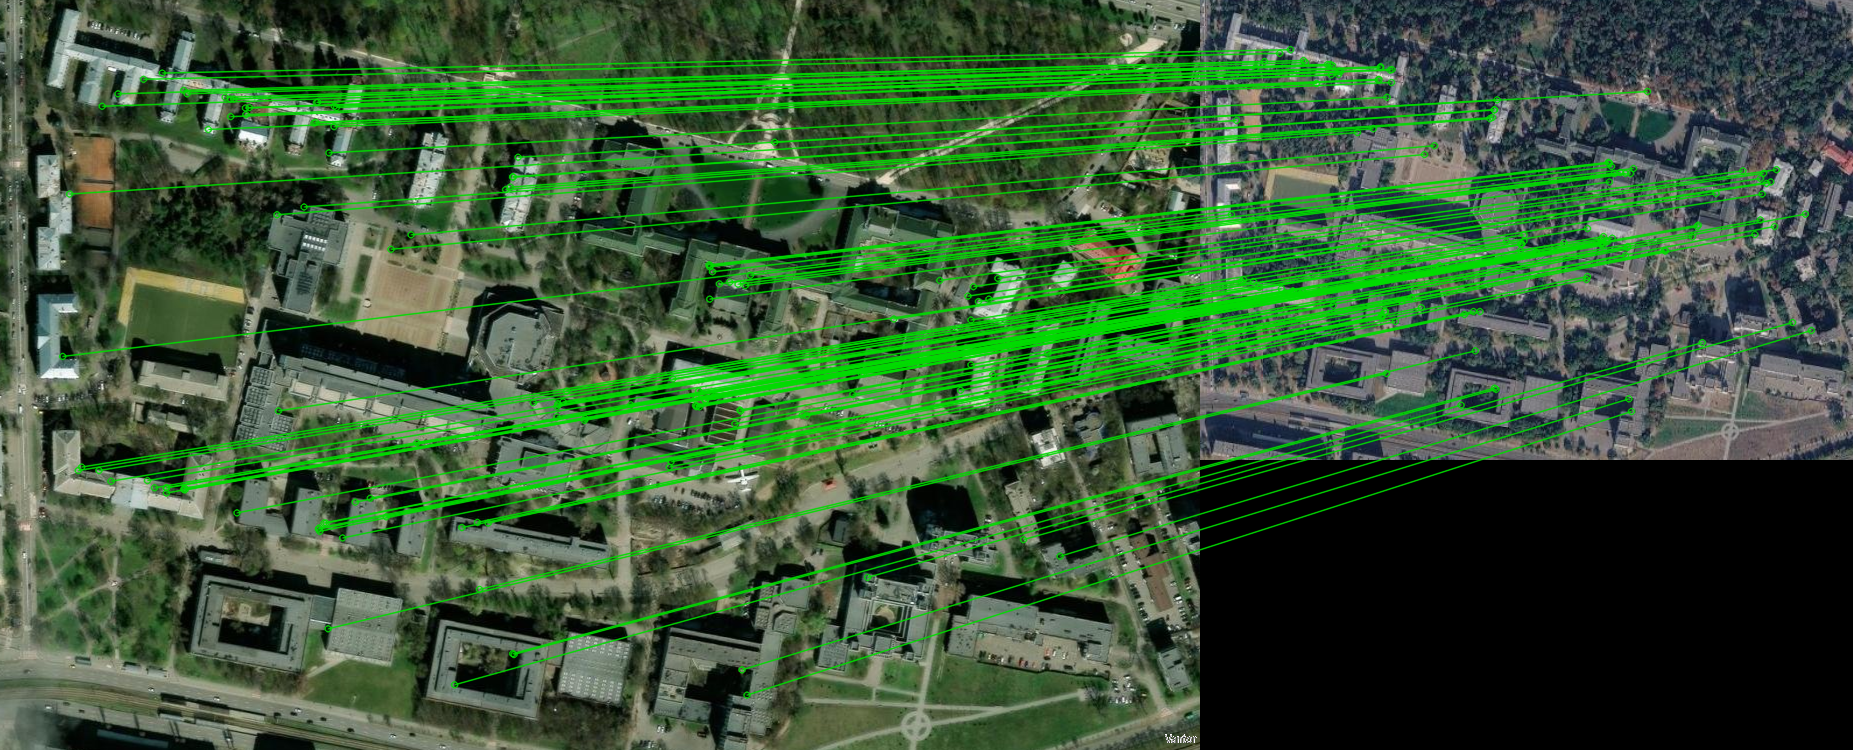
\includegraphics[width=0.98\textwidth]{../results/orb/inlier_matches.png}
  \caption{123 геометрично підтверджені відповідності ORB}
\end{figure}
\begin{figure}[H]\centering
  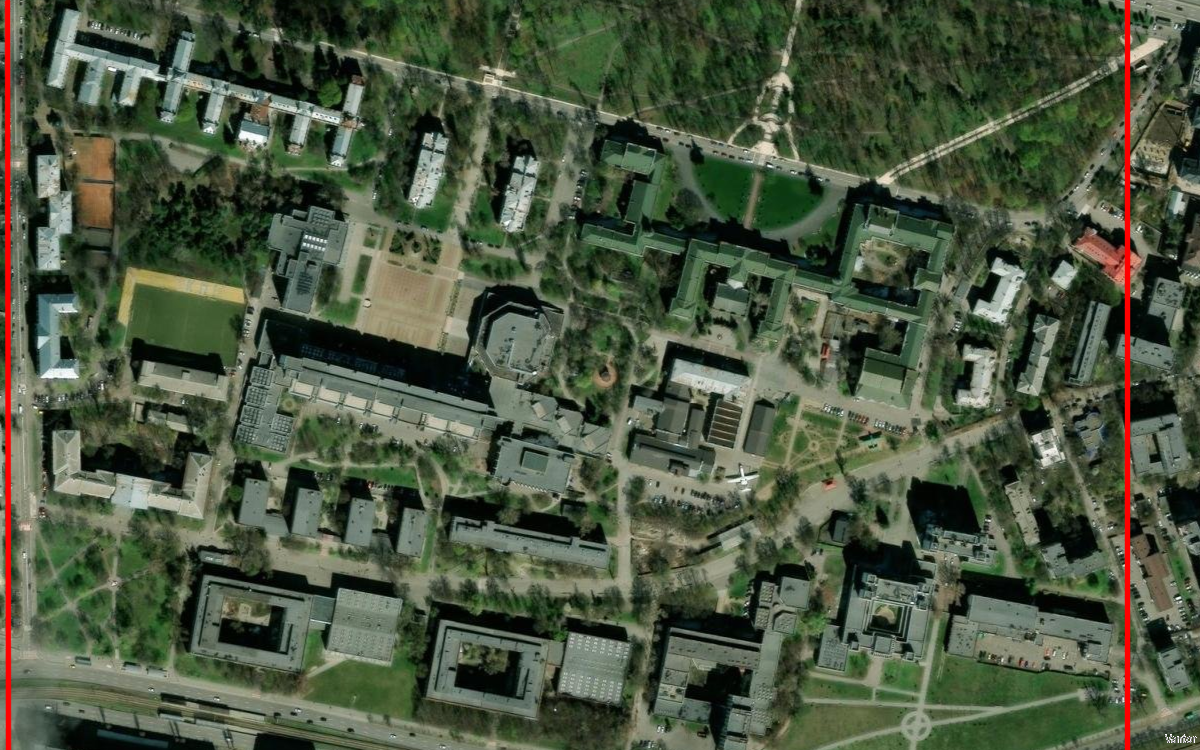
\includegraphics[width=0.96\textwidth]{../results/orb/projected_region.png}
  \caption{Проєкція меж Bing-знімка на Landsat-знімок за оціненою гомографією}
\end{figure}
\begin{figure}[H]\centering
  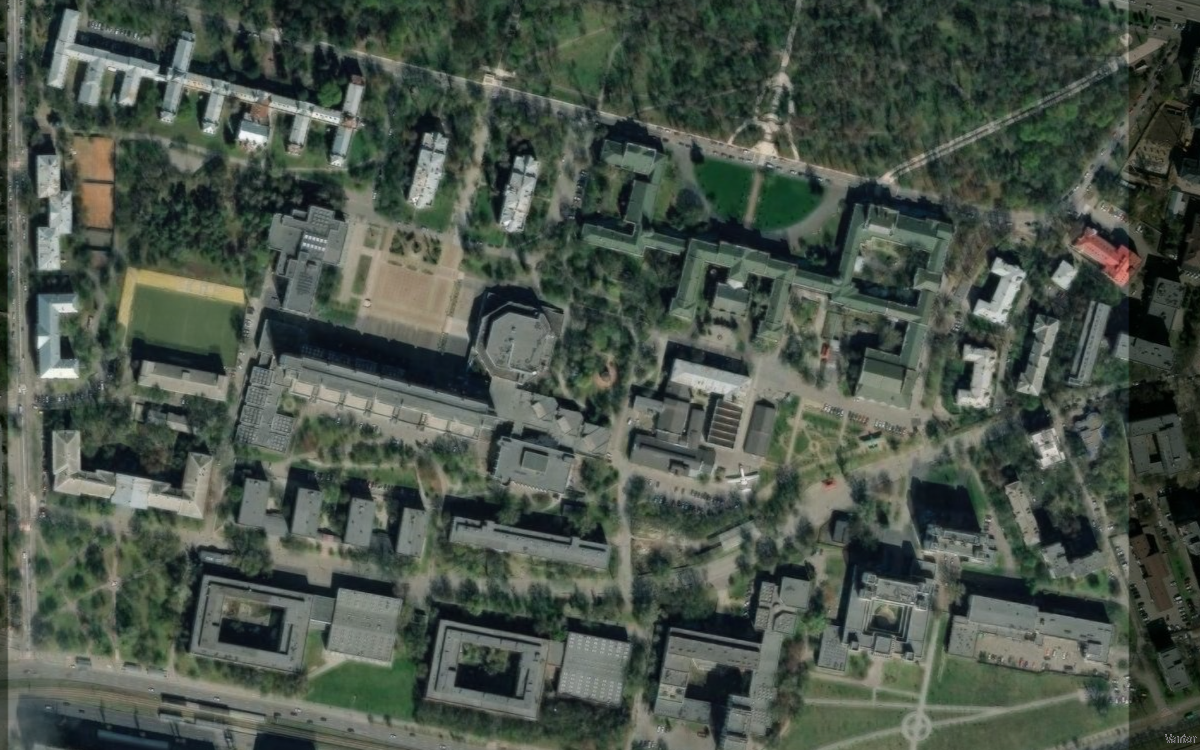
\includegraphics[width=0.96\textwidth]{../results/orb/alignment_blend.png}
  \caption{Контрольне накладання знімків після перспективного вирівнювання}
\end{figure}

Для перевірки відтворюваності виконано повторний запуск із фіксованим seed OpenCV. Для ORB отримано
\begin{equation}
P_{id}^{ORB}=\frac{123}{129}=0{,}9535>0{,}9,
\end{equation}
а для SIFT
\begin{equation}
P_{id}^{SIFT}=\frac{150}{159}=0{,}9434>0{,}9.
\end{equation}
Візуальний контроль показує, що відповідності розподілені по всій спільній частині кампусу, а не зосереджені в одній випадковій локальній області. Контур проєкції та накладання підтверджують правильність оціненої гомографії.

\section{Висновки}
У лабораторній роботі виконано групу вимог 1: порівняно два статичні знімки центральної частини кампусу КПІ з різних джерел, реалізовано попередню обробку, пошук особливих точок, зіставлення дескрипторів, ratio test і геометричну перевірку RANSAC. Досліджено ORB та SIFT.

Для ORB отримано 123 підтверджені відповідності зі 129 придатних та ймовірність ідентифікації $0{,}9535$. Для SIFT отримано 150 зі 159 та $0{,}9434$. Обидва результати перевищують заданий рівень $0{,}9$, тому технічну вимогу виконано. ORB обрано основним методом завдяки вищому значенню метрики й меншій складності бінарних дескрипторів.

\section{Лістинг програми}
\inputminted{python}{../src/main.py}

\end{document}
